\documentclass[
	paper=a4,
	fontsize=11pt,
]{scrartcl}

% Sprache
\usepackage[%
%english,
ngerman
]{babel}
\usepackage[%
plain,
%english,
german
]{fancyref}
\usepackage{setspace}

\usepackage{bibgerm}

% preamble
%% $Id: settings.tex 20568 2010-09-10 14:56:08Z menski $

%%% === Textbody ==============================================================
\KOMAoptions{%
   DIV=11,% (Size of Text Body, higher values = greater textbody)
   % DIV=calc % (also areaset/classic/current/default/last) 
   % -> after setting of spacing necessary!   
   BCOR=5mm% (Bindekorrektur)
}%
%%% === Headings ==============================================================
\KOMAoptions{%
   %%%% headings
	% headings=small,  % Small Font Size, thin spacing above and below
   	% headings=normal, % Medium Font Size, medium spacing above and below
   	headings=big, % Big Font Size, large spacing above and below
   	%
   	%headings=noappendixprefix, % chapter in appendix as in body text
	%headings=nochapterprefix,  % no prefix at chapters
   	% headings=appendixprefix,   % inverse of 'noappendixprefix'
   	% headings=chapterprefix,    % inverse of 'nochapterprefix'
   	% headings=openany,   % Chapters start at any side
   	% headings=openleft,  % Chapters start at left side
   	%headings=openright, % Chapters start at right side      
   	%%% Add/Dont/Auto Dot behind section numbers 
   	%%% (see DUDEN as reference)
   	% numbers=autoenddot
   	% numbers=enddot
   	numbers=noenddot
   	% secnumdepth=3 % depth of sections numbering (???)
}   %
\setcounter{secnumdepth}{3}
%%% === Page Layout ===========================================================
\KOMAoptions{% (most options are for package typearea)
   % twoside=true, % two side layout (alternating margins, standard in books)
   twoside=false, % single side layout 
   % twoside=semi,  % two side layout (non alternating margins!)
   %
   twocolumn=false, % (true)
   %
   headinclude=false,%
   footinclude=false,%
   mpinclude=false,%      
   %
   headlines=2.1,%
	% headheight=2em,%
   headsepline=true,%
   footsepline=false,%
   cleardoublepage=empty %plain, headings
}%
%%% === Paragraph Separation ==================================================
\KOMAoptions{%
	% parskip=relative, % change indentation according to fontsize (recommanded)
   parskip=absolute, % do not change indentation according to fontsize
   parskip=false    % indentation of 1em
   % parskip=true   % parksip of 1 line - with free space in last line of 1em
   % parskip=full-  % parksip of 1 line - no adjustment
   % parskip=full+  % parksip of 1 line - with free space in last line of 1/4
   % parskip=full*  % parksip of 1 line - with free space in last line of 1/3
   % parskip=half   % parksip of 1/2 line - with free space in last line of 1em
   % parskip=half-  % parksip of 1/2 line - no adjustment
   % parskip=half+  % parksip of 1/2 line - with free space in last line of 1/3
   % parskip=half*  % parksip of 1/2 line - with free space in last line of 1em
}%
%%% === Table of Contents =====================================================
\setcounter{tocdepth}{3} % Depth of TOC Display
\KOMAoptions{%
   %%% Setting of 'Style' and 'Content' of TOC
   % toc=left, %
   toc=indented,%
   %
   toc=bib,
   % toc=nobib,
   % toc=bibnumbered,
   %
	% toc=index,%
   toc=noindex,
   %
   % toc=listof,
   toc=nolistof
   % toc=listofnumbered,
   %   
}%  
%%% === Lists of figures, tables etc. =========================================
\KOMAoptions{%
   %%% Setting of 'Style' and 'Content' of Lists 
   %%% (figures, tables etc)
	% --- General List Style ---
   listof=left, % tabular styles
   listof=indented, % hierarchical style
   % --- chapter highlighting ---
   % listof=chapterentry, % ??? Chapter starts are marked in figure/table
   % listof=chaptergapline, % New chapter starts are marked by a gap 
      		  			   	 % of a single line
   %listof=chaptergapsmall, % New chapter starts are marked by a gap 
   	    					   % of a smallsingle line
   % listof=nochaptergap, % No Gap between chapters
   %
   % listof=leveldown, % lists are moved one level down ???
   % --- Appearance of Lists in TOC
   % listof=notoc, % Lists are not part of the TOC
   listof=totoc % add Lists to TOC without number
   % listof=totocnumbered, % add Lists to TOC with number
}%  
%%% === Bibliography ==========================================================
%% Setting of 'Style' and 'Content' of Bibliography
\KOMAoptions{%
	% bibliography=oldstyle,%
   bibliography=openstyle,%
   % bibliography=nottotoc, % Bibliography is not part of the TOC
   % bibliography=totocnumbered, % add Bibliography to TOC with number
   bibliography=totoc % add Bibliography to TOC without number
}%
%%% === Index =================================================================
%% Setting of 'Style' and 'Content' of Index in TOC
\KOMAoptions{%
   index=nottotoc % index is not part of the TOC
	% index=totoc, % add index to TOC without number
}%
%%% === Titlepage =============================================================
\KOMAoptions{%
   titlepage=true %
   %titlepage=false %
}%
%%% === Miscellaneous =========================================================
\KOMAoptions{% 	
   footnotes=multiple% nomultiple
   %open=any,%
   %open=left,%
   %open=right,%
   %chapterprefix=false,%
   %appendixprefix=false,%
   %chapteratlists=10pt,% entry
}%
%% $Id: preamble.tex 20694 2010-09-21 18:47:18Z menski $

%% $Id: preamble-commands.tex 20694 2010-09-21 18:47:18Z menski $

\usepackage{xspace}
\usepackage{ifthen}
\usepackage{ifpdf}

\makeatletter

\providecommand{\IfPackageLoaded}[2]{\@ifpackageloaded{#1}{#2}{}}
\providecommand{\IfPackageNotLoaded}[2]{\@ifpackageloaded{#1}{}{#2}}
\providecommand{\IfElsePackageLoaded}[3]{\@ifpackageloaded{#1}{#2}{#3}}

\def \mail {}
\newcommand{\email}[1]{\def \mail {#1}}

\@ifundefined{frontmatter}{%
   \newcommand{\frontmatter}{%
      %In Roemischen Buchstaben nummerieren (i, ii, iii)
      \pagenumbering{roman}
   }
}{}
\@ifundefined{mainmatter}{%
   % scrpage2 benoetigt den folgenden switch
   % wenn \mainmatter definiert ist.
   \newif\if@mainmatter\@mainmattertrue
   \newcommand{\mainmatter}{%
      % -- Seitennummerierung auf Arabische Zahlen zuruecksetzen (1,2,3)
      \pagestyle{fancy}%%
      \pagenumbering{arabic}%%
   }
}{}
\@ifundefined{backmatter}{%
   \newcommand{\backmatter}{
      %In Roemischen Buchstaben nummerieren (i, ii, iii)
      \pagenumbering{Roman}
   }
}{}

% \def\thickhrulefill{\leavevmode \leaders \hrule height 1pt\hfill \kern \z@}
% \renewcommand{\maketitle}{\begin{titlepage}%
%     \let\footnotesize\small
%     \let\footnoterule\relax
    % \parindent \z@
    % \reset@font
    % \null
    % \vskip 10\p@
    % \hbox{\mbox{%
    %     \hspace{4pt}%
      %   		
\includegraphics[width=7em]{images/uni-logo}%
      %   \hspace{4pt}
      %   }%
      % \vrule depth 0.80\textheight%
      % \mbox{\hspace{2em}}
      % \vtop{% %%%%%%%%%%%%%%%%%%
      %   \vskip 20\p@
        % \begin{flushleft}
        %   \Huge \bfseries \@title \par
        % \end{flushleft}
        % \vskip 60\p@
        % \begin{flushleft}
        %   \LARGE BACHELORARBEIT \par 
        %   \vskip 5\p@
        %   \large zur Erlangung des akademischen Grades\\\Large\textit{Bachelor of Science}\\\large im Studiengang Informatik \par
        %   \vskip 5\p@
        %   \LARGE \@author \par
        %   \vskip 1\p@
        %   \large \mail \par
        % \end{flushleft}
	% 	\vskip 90\p@
        % \begin{flushleft}
        %   \large \@publishers \par
        % \end{flushleft}
        % \vskip 30\p@
        % \begin{flushleft}
        %   \large \@date \par
    %     \end{flushleft}
    %     \vfil
    %     }}        
    % \null
%   \end{titlepage}%
%   \setcounter{footnote}{0}%
% }

%\def\thickhrulefill{\leavevmode \leaders \hrule height 1pt\hfill \kern \z@}
%\renewcommand{\maketitle}{\begin{titlepage}%
%    \let\footnotesize\small
%    \let\footnoterule\relax
%    \parindent \z@
%    \reset@font
%    \null
%    \vskip 10\p@
%    \hbox{\mbox{%
%        \hspace{4pt}%
%			
\includegraphics[width=7em]{images/uni-logo}%
%        \hspace{4pt}
%        }%
%      \vrule depth 0.80\textheight%
%      \mbox{\hspace{2em}}
%      \vtop{% %%%%%%%%%%%%%%%%%%
%        \vskip 20\p@
%        \begin{flushleft}
%          \Huge \bfseries \@title \par
%          \LARGE \bfseries \@subtitle \par
%        \end{flushleft}
%        \vskip 60\p@
%        \begin{flushleft}
%          \LARGE Bachelor Thesis \par 
%          \vskip 5\p@
%          \large by \par
%          \vskip 5\p@
%          \LARGE \@author \par
%          \vskip 1\p@
%          \large \mail \par
%        \end{flushleft}
%		\vskip 120\p@
%        \begin{flushleft}
%          \large \@publishers \par
%        \end{flushleft}
%        \vskip 30\p@
%        \begin{flushleft}
%          \large \@date \par
%        \end{flushleft}
%        \vfil
%        }}        
%    \null
%  \end{titlepage}%
%  \setcounter{footnote}{0}%
%}

\makeatother

% Encoding
\usepackage[T1]{fontenc}
\usepackage[%
%	latin1,
	utf8
]{inputenc}

% Layout
\usepackage{fancyhdr}

% Refernces
\usepackage[]{prettyref}
%\newrefformat{cha}{Kapitel \ref{#1}}
%\newrefformat{sec}{Abschnitt \ref{#1}}
%\newrefformat{tab}{Tabelle \ref{#1} auf Seite \pageref{#1}}
%\newrefformat{fig}{Abbildung \ref{#1} auf Seite \pageref{#1}}
%\newrefformat{fig}{Abbildung \ref{#1}}
\newrefformat{fig}{Figure \ref{#1}}
%\newrefformat{lst}{Listing \ref{#1} auf Seite \pageref{#1}}

\usepackage{todonotes}

% Grafik
% \usepackage[%
% 	table
% ]{xcolor}
\usepackage{graphicx}
\usepackage{epstopdf}

% Mathe
\usepackage[%
	centertags,
	sumlimits,
	intlimits,
	namelimits,
	fleqn
]{amsmath}
\usepackage[
	all,
	warning
]{onlyamsmath}
\usepackage{fixmath}

\usepackage{tikz}
\usetikzlibrary{arrows}

% Berechnungen
\usepackage{calc}

% Textauszeichnung
\usepackage{soul}
\usepackage[normalem]{ulem}
\usepackage{url}
\usepackage[%
	babel,
	german=quotes,
	english=british
]{csquotes}
\usepackage{ragged2e}
\usepackage{multicol}
\usepackage[
	colorlinks=false,
	pdfborder={0 0 0},
]{hyperref}

% Floats
\usepackage{float}
\usepackage{flafter}
\usepackage[%
	section,
	above
]{placeins}
%\usepackage[lofdepth=2]{subfig}
\usepackage{subcaption}
\usepackage{wrapfig}
\setlength{\intextsep}{0.5\baselineskip}

% Tabellen
\usepackage{booktabs}
\usepackage{multirow}
\usepackage{dcolumn}
\usepackage{ltxtable}

% Wissenschaft
\usepackage{units}

% Listings
%\usepackage{algorithmic}
%\usepackage{algorithm}
\usepackage[ruled,vlined,linesnumbered]{algorithm2e}
\usepackage{listings}
\lstset{ %
language=,                % choose the language of the code
basicstyle=\footnotesize,       % the size of the fonts that are used for the code
numbers=none,                   % where to put the line-numbers
numberstyle=\footnotesize,      % the size of the fonts that are used for the line-numbers
stepnumber=1,   	            % the step between two line-numbers. If it's 1 each line
                                % will be numbered
numbersep=5pt,                  % how far the line-numbers are from the code
backgroundcolor=\color{white},  % choose the background color. You must add \usepackage{color}
showspaces=false,               % show spaces adding particular underscores
showstringspaces=false,         % underline spaces within strings
showtabs=false,                 % show tabs within strings adding particular underscores
%frame=single,	                % adds a frame around the code
tabsize=2,	                % sets default tabsize to 2 spaces
captionpos=b,                   % sets the caption-position to bottom
breaklines=true,                % sets automatic line breaking
breakatwhitespace=false,        % sets if automatic breaks should only happen at whitespace
%title=\lstname,                 % show the filename of files included with \lstinputlisting;
                                % also try caption instead of title
escapeinside={\%*}{*)},         % if you want to add a comment within your code
morekeywords={*,...}            % if you want to add more keywords to the set
}


%%% Local Variables:
%%% mode: latex
%%% TeX-master: "../master"
%%% End:

\usepackage[absolute]{textpos}

\newlength{\TitleLeft}
\newlength{\TitleRight}
\newlength{\TitleAbove}
\newlength{\TitleWidth}

\setlength{\TitleLeft}{2cm}
\setlength{\TitleRight}{2cm}
\setlength{\TitleAbove}{2cm}
\setlength{\TitleWidth}{\paperwidth-\TitleLeft-\TitleRight}

\newcommand{\BAUni}{Universität~Potsdam}
\newcommand{\BAInstitut}{Mathematisch-Naturwissenschaftliche~Fakultät\\Institut~für~Informatik}
\newcommand{\BABetreuerText}{Betreuer}
\newcommand{\BAAutor}{Sebastian~Menski (734272)\\menski@uni-potsdam.de}
\newcommand{\BATyp}{Projektarbeit}
\newcommand{\BAAbschlussText}{}
\newcommand{\BAAbschluss}{}
\newcommand{\BATitle}{tcpdump Analyse}
\newcommand{\BABetreuer}{Dipl.-Inf. Simon Kiertscher}
\newcommand{\BAOrt}{Potsdam}
\newcommand{\BAAbgabedatum}{16. Mai 2016}

\definecolor{uniblue}{rgb}{0.062745,0.17647,0.34118}

\renewcommand{\maketitle}{
  \thispagestyle{empty}
  \begin{textblock*}{\TitleWidth}(\TitleLeft,\TitleAbove)
    ~\hfill
\includegraphics[height=2.5cm]{images/uni-logo}\\[3mm]
    {\color{uniblue}\rule{\TitleWidth}{1mm}}\\[5mm]
    {
      \centering
      \sffamily\Large
      {\LARGE\BAUni}\\[0.5\baselineskip]
      {\large\BAInstitut}\\[4\baselineskip]
      {\BATyp}\\[\baselineskip]
      {\Huge\BATitle}\\[6\baselineskip]

      \BAAutor\\[7\baselineskip]
      \begin{tabular}{rl}
         \BABetreuerText: & \BABetreuer
      \end{tabular}\\[3\baselineskip]
      \BAOrt, \BAAbgabedatum\par
    }
  \end{textblock*}
  ~\clearpage
}


% macros
% % FancyRef
\newcommand*{\fancyrefalglabelprefix}{alg}
\newcommand*{\Frefalgname}{Algorithm}
\newcommand*{\frefalgname}{\MakeLowercase{\Frefalgname}}
\frefformat{main}{\fancyrefalglabelprefix}{%
  \textbf{\frefalgname\fancyrefdefaultspacing#1}#3}
\frefformat{vario}{\fancyrefalglabelprefix}{%
  \frefalgname\fancyrefdefaultspacing#1#3}
\frefformat{plain}{\fancyrefalglabelprefix}{%
  \frefalgname\fancyrefdefaultspacing#1}

% \newcommand{\marginnote}[1]{\marginpar{
% \raggedright\footnotesize
% \itshape#1\par}}
% \newcommand{\todo}[1]{\marginnote{\textbf{TODO:}#1}}

%%% Local Variables: 
%%% mode: latex
%%% TeX-master: "../master"
%%% End: 


\hypersetup{
  pdfauthor = {Sebastian Menski},
  pdftitle = {\BATitle},
}

\begin{document}
%% FRONTMATTER
\frontmatter
\maketitle
\clearpage

\tableofcontents
%\listoftodos
%% MAINMATTER
\clearpage
\mainmatter
\onehalfspacing
\section{Einleitung}
\label{sec:einleitung}

Diese Arbeit untersucht ob tcpdump\footnote{\url{http://www.tcpdump.org/}} zum
Monitoren von HTTP Traffic in einem Hochlastszenario geeignet ist. Der Use
Case ist, dass tcpdump dazu eingesetzt werden soll HTTP Traffic zu überwachen
und zu analysieren. Anhand der gewonnen Daten sollen Entscheidungen getroffen
werden um eine Lastverteilungsinfrastruktur zu steuern. Um dies sinnvoll
einzusetzen muss sichergestellt werden, dass das Monitoring alle oder
mindestens den größten Teil der HTTP Requests aufzeichnen kann.

Um in diesem Kontext tcpdump zu evaluieren wird diese Arbeit zuerst die
Grundlagen von tcpdump im Kapitel \ref{sec:grundlagen} erklärt. Dabei wird
gezeigt wie tcpdump Pakete filtert und wo es dort zu Paketverlusten kommen
kann. Anschließend werden in Kapitel \ref{sec:verwandte-arbeiten} Arbeiten
aufgeführt die sich bereits mit der Performance von tcpdump beschäftigt haben.
Das Kapitel \ref{sec:konzept} beschreibt dann den Versuchsaufbau für diese Arbeit
und was dabei die erwarteten Beobachtungen sind. Die Messergebnisse der
Experimente werden in Kapitel \ref{sec:messungen} vorgestellt und ausgewertet.
Das letzte Kapitel \ref{sec:zusammenfassung} gibt eine Zusammenfassung der
Ergebnisse dieser Arbeit und eine Einschätzung ob tcpdump in dem beschrieben
Use Case sinnvoll eingesetzt werden kann.

Die Beschreibungen und Messungen in dieser Arbeiten basieren alle auf der tcpdump
Version 4.3.0 und der dazu gehörigen libpcap Version 1.3.0. Das Betriebssystem
auf dem tcpdump lief war Centos 5 mit einem Kernel der Version 2.6.18.

Diese Arbeit befasst sich nur mit der Paketaufzeichnung und nicht mit der
Weiterverarbeitung und Auswertung der aufgezeichneten Daten.

\clearpage
\section{Grundlagen}
\label{sec:grundlagen}

Tcpdump\footnote{\url{http://www.tcpdump.org/}} ist eine Software um
Netzwerkpakete aufzuzeichnen. Tcpdump benutzt die Bibliothek libpcap, welche
eine einheitliche API anbieten um Netzwerkpakete auf unterschiedlichen
Betriebssystemen aus dem Netzwerkverkehr herauszufiltern. Ziel hierbei ist es
Paket möglichst früh im Netzwerkstack zu filtern, wodurch nur Pakete
von Interesse weiterverarbeitet werden müssen.

Diese Kapitel beschreibt wie tcpdump/libpcap in Linux Netzwerkpakete filtert.
Dazu wird wie in
\cite{Insolvibile:2001:KKL,Insolvibile:2002:KKIa,Insolvibile:2002:KKIb}
beschrieben der Verlauf eines eingehenden TCP Paketes durch den Linux Kernel
betrachtet.


\begin{figure} \centering

\includegraphics[width=.7\textwidth]{images/network-stack.eps}
\caption{Schematischer Paketfluss beim Empfang eines TCP Paketes im Linux
Kernel}\label{fig:network-stack}
\end{figure}

In Abbildung~\ref{fig:network-stack} sind die wichtigsten Teile des Linux
Networkstacks dargestellt, welche bei dem Empfang eines TCP Paketes eine Rolle
spielen. Im Userspace wird ein Webserver (nginx) betrieben, welcher über einen
TCP Socket HTTP Requests empfängt. Parallel läuft tcpdump/libpcap welches einen
speziellen \texttt{PF\_PACKET} Socket nutzt um alle empfangen Pakete zu
untersuchen (siehe Listing~\ref{lst:pfpacket}).

\begin{lstlisting}[caption={Erzeugen eines \texttt{PF\_PACKET} Sockets},label=lst:pfpacket]
socket(PF_PACKET, SOCK_RAW, htons(ETH_P_ALL));
\end{lstlisting}


Ein solcher Socket ermöglicht es Pakete direkt von der Netzwerkkarte zu
erhalten ohne das die Pakete den normalen Netzwerkstack durchlaufen, dies ist
wichtig für tcpdump da es das komplette Paket aufzeichnen will.

Erreicht ein TCP Paket die Netzwerkkarte wird es zuerst in eine Queue in der
Netzwerkkarte (1) abgespeichert. Anschließend wird das Paket in die zuständige
CPU Eingangsqueue übergeben (2). Danach übernimmt die Kernel Funktion
\texttt{net\_rx\_action} die Weitergabe des Paketes. Dazu werden zwei Listen
von Handler betrachtet. Als erstes wird das Paket an alle Handler übergeben,
welche alle Pakete empfangen. Dazu zählt auch der \texttt{PF\_PACKET} Socket
von tcpdump/libpcap. Anschließend werden spezielle Handler für das Paket
aufgerufen. In dem Fall eines TCP Paketes ist dies der IP Handler, welcher den
IP Header liest, auswertet und entfernt.  Anschließend wird das Paket an den
TCP Handler übergeben. Dieser wertet den TCP Header aus und reicht das Paket an
den zuständigen Socket weiter. Wenn ein Paket einen Socket erreicht wird es in
dessen Eingangsbuffer (3) abgelegt.

Wie in Abbildung~\ref{fig:network-stack} zu sehen ist, gibt es mindestens drei
Paketbuffer die ein Paket durchläuft. Wenn einer dieser Buffer voll ist, weil
bereits zu viele Paket angenommen aber nicht verarbeitet wurden, wir ein neues
Paket verworfen. Unter der Fragestellung unter welchen Umständen tcpdump Pakete
verwirft, welcher allerdings die Anwendung (nginx) erreichen, sind die ersten
beiden Buffer (NIC und CPU Queue) nicht interessant. Ein Paket, welches bereits
an dieser Stelle verworfen wird, erreicht weder die Anwendung noch tcpdump.
Insofern ist nur der dritte Buffer vom Socket interessant. An dieser Stelle hat
das Paket bereits zwei unterschiedliche Wege durchlaufen. Dabei muss die Anzahl
der Paket in beiden Sockets nicht identisch sein, da der \texttt{PF\_PACKET}
generell alle Pakete erhält. Dies bedeutet, wenn neben dem HTTP Verkehr noch
weiterer Netzwerkverkehr existiert wird dieser ebenfalls an den tcpdump/libpcap
Socket weitergeleitet.

Daher ist es nötig diesen Traffic möglichst frühzeitig zu filtern. Eine
Filterung im Userspace würde das Problem nicht beheben, da immer noch alle
Pakete erst einmal den Socket erreichen. Linux stellt für diese Zweck den Linux
Socket
Filter\footnote{\url{https://www.kernel.org/doc/Documentation/networking/filter.txt}}
(LSF) bereit. Diese API wurde mit Kernel 2.2 einführt und ermöglicht es ein Filter
an einem Socket zu registrieren (siehe Listing~\ref{lst:attach}).

\begin{lstlisting}[caption={Anhängen eines Filters an eine Socket},label=lst:attach]
setsockopt(socket, SOL_SOCKET, SO_ATTACH_FILTER, filter, sizeof(*filter));
\end{lstlisting}

Der Filter ist ein Programm in der Assembler ähnlichen Sprache Berkley Paket
Filter (BPF)~\cite{DBLP:conf/usenix/McCanneJ93}. Die Sprache umfasst einfache
Vergleich- und Rechenoperation und arbeitet direkt auf den Daten des
Netzwerkpaketes. Dadurch kann der Filter direkt auf einzelne Header Felder
der verschieden Protokolle zugreifen.\ tcpdump/libpcap erlaubt es logische
Ausdrücke zum erstellen eines Filters in BPF umzuwandeln. Das Beispiel
in Listing~\ref{lst:filter} zeigt den BPF Code für einen Filter der alle
TCP Pakete für die Ziel-IP \texttt{10.3.9.21} und Ziel-Port \texttt{80} akzeptiert.

\begin{lstlisting}[numbers=none,caption={BPF for \texttt{tcpdump -d ip dst host 10.3.9.21 and tcp dst port 80}},label={lst:filter}]
(000) ldh      [12]
(001) jeq      #0x800           jt 2    jf 12
(002) ld       [30]
(003) jeq      #0xa030915       jt 4    jf 12
(004) ldb      [23]
(005) jeq      #0x6             jt 6    jf 12
(006) ldh      [20]
(007) jset     #0x1fff          jt 12   jf 8
(008) ldxb     4*([14]&0xf)
(009) ldh      [x + 16]
(010) jeq      #0x50            jt 11   jf 12
(011) ret      #65535
(012) ret      #0
\end{lstlisting}

Das BPF Programm lädt Daten aus dem Netzwerkpaket und vergleicht diese mit dem
festgelegten Filter. Zuerst wird der EtherType aus dem Ethernet Header geladen
(000) und verglichen ob es sich um ein IPv4 Paket (Type: 0x0800) handelt (001).
Ist der Vergleich erfolgreich wird mit der nächsten Instruktion fortgefahren,
ansonsten wird zu letzten Instruktion (012) gesprungen. Als zweites wird die
Ziel-Adresse aus dem IP Header geladen (003) und mit der IP 10.3.9.21
(0xa030915) verglichen (004). Danach wird das Protokolfeld des IP Headers
geladen (004) und überprüft, dass es sich um ein TCP Paket (0x6) handelt (005).
In der folgende Instruktion wird sichergestellt, dass das IP Paket nicht
fragmentiert wurde oder es sich um das erste Fragment handelt, also der IP
Fragment Offset 0 ist (007). Anschließend wird die IP Headerlänge im
Hilfsregister X gespeichert (008), dies ist nötig, da der IP Header durch
Optionen eine variable Länge besitzt. Ein Zugriff auf den TCP Header ist nur
mit dieser Information möglich. Als letztes wird der Ziel-Port aus dem TCP
Header geladen (009) und mit Port 80 (0x50) verglichen (010). Wenn alle diese
Tests erfolgreich waren wird mit Instruktion (011) das Paket akzeptiert.
Ansonsten wird das Paket mit Instruktion (012) abgelehnt. Das BPF Programm gibt
die Anzahl der Bytes zurück, welche von dem Paket weitergeleitet werden sollen.
In libpcap ist der Standard dafür 65535 Bytes (siehe Instruktion 011), welches
die maximale Größe eines IP Paketes entspricht. Der Rückgabewert 0 gibt an
das kein Byte des Paketes weitergegeben werden soll (012).

Ist ein Filter für einen Socket registriert, wird dieser vom Handler durch die Kernel
Funktion \texttt{sk\_run\_filter} ausgeführt, bevor
das Paket an den Socket übergeben wird. Dadurch kann die Anzahl der Paket,
welche den tcpdump/libpcap Socket erreichen effizient reduziert werden.

Der tcpdump/libpcap Socket Buffer wird als Memory Mapped Packet Ring
Buffer\footnote{\url{https://www.kernel.org/doc/Documentation/networking/packet_mmap.txt}}
angelegt. Dies ermöglicht es effizienter auf Paket im Userspace zu zugreifen.
Dies verhindert, dass jedes Paket einzeln durch einen \texttt{recv} Aufruf
empfangen werden muss.  Die Größe des Buffers ist standardmäßig 2~MB\@. Der
Buffer wird in Frames aufgeteilt, welche es ermöglichen das aufgezeichnete
Paket und Metadaten zu speichern. Dabei richtet sich die Framegröße nach der
Anzahl der Bytes die pro Paket aufgezeichnet werden.

Es zeigt sich, dass es mindestens drei Merkmale gibt, welche beeinflussen wieviel
Paket tcpdump/libpcap aufzeichnen kann. Dies ist zu erst der Filter welcher
möglichst viele Paket bereits im Kernel verwerfen sollte. Anschließend die
Anzahl der Bytes die pro gefiltertem Paket weitergegeben werden und die
Buffergröße die verwendet wird um die Paket vorzuhalten. Die Auswirkung
dieser Aspekte soll in dieser Arbeit mit Hilfe von Messungen untersucht werden.
Außerdem ist bereits aus Abbildung~\ref{fig:network-stack} ersichtlich das die
Ausführung von tcpdump eine Auswirkung auf andere Services hat, da jedes Paket
nun von einem zusätzlichen Handler betrachtet und gefiltert wird. Daher hat die
Komplexität und Effektivität des tcpdump Filters einen direkten Einfluss auf
die Geschwindigkeit mit der Paket verarbeitet werden.

\clearpage
\section{Verwandte Arbeiten}
\label{sec:verwandte-arbeiten}

In \cite{schneider05da,DBLP:conf/conext/SchneiderW05} wurde untersucht ob sich
nicht spezialisierte Hardware zum Aufzeichnen von Paketen in Gigabit Netzwerken
eignet. Es wurden 4 verschieden Systeme verglichen, welche sich nur in der
verwendeten CPU und dem Betriebssystem unterschieden. Als CPUs wurden AMD
Opteron und Intel Xeon verwendet. Die Betriebssysteme waren Linux 2.6.11 und
FreeBSD 5.4. In den Messungen wurde der Linux Kernel Package Generator
\cite{DBLP:journals/comcom/TurullSO16} genutzt um UDP Pakete zu generieren. Die
Paketgrößen wurde anhand einer Verteilung generiert, welche aus einer 24h
Aufzeichnung abgeleitet wurde. Die Ergebnisse der Experimente zeigten, dass mit
steigender Paketrate die CPU Auslastung und der Paketverlust bei der
Aufzeichnung steigt. Außerdem zeigte sich das die Kombination aus FreeBSD und
AMD Opteron den geringsten Paketverlust aufzeigte. In einer anknüpfenden Arbeit
\cite{DBLP:conf/pam/SchneiderWF07} wurden Ansätze beschrieben wie man höhere
Netzwerkarten wie 10-Gigabit Ethernet auf mehrere 1-Gigabit Interfaces
verteilen kann. Dadurch kann der erhöhte Netzwerkverkehr immer noch effizient
aufgezeichnet werden.

Den Einfluss von tcpdump auf die Leistung eines parallel laufenden Dienstes,
wie zum Beispiel einem Webserver, wurde in \cite{DBLP:conf/globecom/ChenCCM11}
untersucht. Es zeigte sich eine starke Beeinträchtigung, wenn sich
tcpdump und der Webserver eine CPU geteilt haben. Allerdings war auch bei
getrennten CPUs die Leistung des Webservers beeinträchtigt.

Technologien wie Intel Data Plane Development
Kit\footnote{\url{http://dpdk.org/}} (DPDK) and
WireCAP\footnote{\url{http://wirecap.fnal.gov/}} \cite{DBLP:conf/imc/WuD14}
untersuchen neue Ansätze um die Paketverarbeitung und -aufzeichnung zu
optimieren.  Dabei stehen Multi-Core Unterstützung und optimierte
Speicherverwaltung im Vordergrund.  Dabei können in Hochlastszenarien
Verbesserungen zu normalen libpcap Anwendungen erzielt werden.

Die existierende Literatur zeigt, dass das Problem des Paketverlustes bei
der Aufzeichnung von Netwerkverkehr unter hoher Last ein bekanntes Problem
ist. Dabei haben viele Faktoren einen Einfluss auf die Paketaufzeichnung. Dies
umfasst die verwendete Hardware, wie Netzwerkkarten, CPU und Festplatten, aber
auch das verwendete Betriebssystem und Software. Da diese Arbeit sich explizit
mit tcpdump/libpcap auf einem gegeben System befasst, wird im folgenden Kapitel
ein Konzept vorgestellt um die Auswirkungen der in Kapitel \ref{sec:grundlagen}
vorgestellten Aspekte von tcpdump/libpcap zu untersuchen.


\clearpage
\section{Konzept}
\label{sec:konzept}

Um die Leistung von tcpdump zur Aufzeichnung von HTTP Traffic zu zeigen wurden
im Rahmen dieser Arbeit mehrere Messungen vorgenommen. Dieses Kapitel beschreibt
das Konzept und den Aufbau dieser Messungen. Und begründet die Entscheidungen
bezüglich der einzelne Komponenten.

Für die Messung standen zwei identische Systeme \texttt{ib5} und \texttt{ib6}
zur Verfügung. Dabei wurde \texttt{ib5} als Benchmark Client und \texttt{ib6}
als System unter Last (SUT) genutzt.

\begin{description}
\item [ib5/ib6] \hfill
\begin{description}
\item [CPU] Quad Core Intel Xeon 2.27 GHz
\item [RAM] 6 GB
\item [OS] CentOS 5.8
\item [Kernel] 2.6.18-308.el5
\item [NIC Treiber] bnx2 2.1.11
\end{description}
\end{description}

Als HTTP Benchmark wurde \texttt{wrk}\footnote{\url{https://github.com/wg/wrk}}
Version 4.0.2 auf \texttt{ib5} genutzt. Dieser Benchmark nutzt Multithreading
und Event Loops um eine möglichst hohe Anzahl an HTTP Requests an das SUT zu
schicken. Auf \texttt{ib6} wurde
\texttt{nginx}\footnote{\url{http://nginx.org/}} Version 1.9.15 als HTTP Server
eingesetzt. Zur Aufzeichnung der Netzwerkpakete wurde
\texttt{tcpdump}\footnote{\url{http://www.tcpdump.org/}} Version 4.3.0 und
\texttt{libpcap} Version 1.3.0 verwendet.

Ziel des Messaufbau war es eine möglichst hohe Anzahl an HTTP Requests zu
erzeugen um eine hohe Last auf tcpdump zu generieren. Um dies zu erreichen
wurden minimal HTTP Requests und Responses genutzt. Dazu wurde nginx so
konfiguriert das es auf einen HTTP GET Requests direkt mit einem 204 No Content
Response antwortet (siehe Listing~\ref{lst:nginx} in
Anhang~\ref{sec:konfigurationen}).  Dies entspricht zwar keinem realen
Szenario, allerdings kann eine reale Überlastsituation nicht mit der vorhanden
Hardware simuliert werden. Es ist jedoch vorstellbar das die Anzahl der Pakete
die durch diese Vereinfachung versendet wurden in einem realen Lastszenario
erreicht werden können. Und eine geringere Last keine Probleme für tcpdump
dargestellt hätten.

\begin{lstlisting}[caption={Aufruf von wrk},label=lst:wrk]
wrk -t 4 -c 1024 -d 5m http://ib6
\end{lstlisting}

\begin{table}
  \centering
  \bgroup
  \def\arraystretch{1.3}
  \begin{tabular}{ccccp{7.6cm}}
      & \textbf{Name} & \textbf{snaplen} & \textbf{buffer} & \textbf{filter} \\\hline\hline
      1 & no & \multicolumn{3}{c}{---} \\\hline
      2 & default & 65535 & 2048 & ip dst host 172.16.0.26 and tcp dst port 80 \\\hline
      3 & snaplen & 142 & 2048 & ip dst host 172.16.0.26 and tcp dst port 80 \\\hline
      4 & buffer  & 65535 & 4096 & ip dst host 172.16.0.26 and tcp dst port 80 \\\hline
      5 & snaplen+buffer & 142 & 4096 & ip dst host 172.16.0.26 and tcp dst port 80 \\\hline
      6 & filter  & 142 & 4096 & ip dst host 172.16.0.26 and tcp dst port 80 and \\
        &      & & & 'tcp[((tcp[12:1] \& 0xf0) >> 2):4] = 0x47455420' \\
  \end{tabular}
  \egroup
  \caption{Konfiguration von tcpdump für Messszenarien}\label{tab:szenarien}
\end{table}

Um die in Kapitel~\ref{sec:grundlagen} aufgeführten Einstellungen von tcpdump
zu untersuchen wurde insgesamt 6 Messreihen durchgeführt. Es wurde Untersucht
wie sich tcpdump allgemein auf die Performance des Webservers auswirkt. Und wie
sich die Parameter Größe der aufgezeichneten Pakete (snaplen), Größte des
Paketbuffers (buffer) und der verwendete Paketfilter (filter) auf tcpdump
auswirken. Bei allen Messungen war die nginx Konfiguration gleich (siehe
Listing~\ref{lst:nginx} in Anhang~\ref{sec:konfigurationen}).  Ebenfalls
wurde wrk immer wie in Listing~\ref{lst:wrk} gezeigt aufgerufen. Jede Messung
war 5 Minuten lang und benutzt 4 Threads und 1024 Verbindungen. Die
Konfiguration von tcpdump wurde für jede Messung angepasst (siehe
Tabelle~\ref{tab:szenarien}). Im Folgenden sollen die einzelnen Szenarien
beschrieben werden.

\paragraph{no} Die erste Messreihe ist eine Kontrollmessung ohne tcpdump. Diese
Messung soll die maximale Anzahl der Requests in der Messumgebung ermitteln.
Anhand dieser Messung können dann Aussagen über den Einfluss von tcpdump auf
die Leistung des HTTP Servers getroffen werden.

\paragraph{default} Bei dieser Messungen wurde die Standardparameter von tcpdump
verwendet. Dabei ist die snaplen 65535 Bytes und der buffer 2048 KBytes. Der Filter
beschreibt alle TCP Pakete für die Ziel-Adresse \texttt{172.16.0.26} und dem Ziel-Port
\texttt{80}. Dies umfasst alle eingehenden TCP Pakete für den Webserver.

\paragraph{snaplen} In diesem Szenario wurden die snaplen auf 142 Bytes
reduziert. Die ersten 142 Bytes eines TCP Paketes reichen aus um zu analysieren
ob es sich um ein HTTP Paket handelt.  Dabei ergibt sich 142 Bytes aus der Mac
Header Größe (14 Bytes), der maximalen IP Header Größe (60 Bytes), der
maximalen TCP Header Größe (60 Bytes) und den ersten 8 Bytes der TCP Payload
(HTTP Methode). Diese Aufzeichnungsgröße ist ausreichend um zu analysieren
wieviel HTTP Pakete den Webserver erreichen, was dem untersuchten Use Case
entspricht. Da für den IP und TCP Header die maximalen Größen angenommen
wurden, werden vermutlich die meisten aufgezeichneten Pakete noch weitere
Informationen wie den Request Pfad enthalten.

\paragraph{buffer} In diesem Szenario wurde die Buffergröße auf 4096 Bytes
verdoppelt, dies sollte es tcpdump ermöglichen mehr Pakete für die
Weiterverarbeitung vorzuhalten.

\paragraph{snaplen+buffer} Diese Szenario kombiniert die Szenarien
\texttt{snaplen} und \texttt{buffer} um die Anzahl der Pakete welche in den
tpcdump Buffer passen zu maximieren.

\paragraph{filter} Das letzte Szenario soll die Auswirkung des gewählten
Filters untersuchen. Dazu wurde der Filter noch einmal verfeinert. Der Filter
für Ziel-IP und Ziel-Port akzeptiert sowohl HTTP Requests als auch TCP Pakete
welche zum Verbingungsaufbau und -abbau gesendet werden. Um diese bereits im
Kernel herauszufiltern wurde der Filter um den Ausdruck \texttt{tcp[((tcp[12:1]
\& 0xf0) >> 2):4] = 0x47455420} erweitert. Dieser Filter testet ob die ersten 4
Bytes der TCP Payload \glqq{}\texttt{GET }\grqq{} entsprechen.  Der
Filter akzeptiert also nur Pakete die GET HTTP Requests sind. Außerdem wurden
die snaplen und buffer Größe vom \texttt{snaplen+buffer} Szenario übernommen.

Jede Messung wurde 7 mal wiederholt. Dabei wurden die Ausgaben von
wrk und tcpdump aufgezeichnet und ausgewertet. Die folgenden Metriken
wurden dann untersucht:

\begin{enumerate}
\item Anzahl der gesendeten HTTP Requests (wrk)
\item Anzahl der gefilterten Netzwerkpakete (tcpdump)
\item Anzahl der verlorenen Netzwerkpakete (tcpdump)
\end{enumerate}

Es wurde erwartet, dass anhand der Ergebnisse gezeigt werden kann, dass tcpdump
eine Auswirkung auf die Anzahl der gesendeten HTTP Requests hat. Außerdem
das es bereits in diesem einfach Messaufbau mit nur einem Client zu Paketverlusten
kommt. Diese jedoch durch eine Anpassung der tcpdump Parameter snaplen und buffer
reduziert werden können. Weiterhin ist die Vermutung, dass ein sehr spezifischer
Filter eine weitere Verbesserung ermöglicht. Das folgende Kapitel~\ref{sec:messungen}
beschreibt die Ergebnisse der einzelnen Messungen und wertet diese aus.

\clearpage
\section{Messungen}
\label{sec:messungen}

Dieses Kapitel stellt die Messergebnisse vor und analysiert diese. Vor der
Messungen wurden keine Änderungen an den Systemkonfigurationen durchgeführt,
außer die maximale Anzahl an offenen Dateien auf 4096 erhöht. Eine Auflistung
der restlichen Limits und die Konfiguration der Netzwerkkarte sind in
Anhang~\ref{sec:konfigurationen} in den Listings~\ref{lst:ulimit}
und~\ref{lst:ethtool} zu finden. Die Messungen wurden durch ein Skript
automatisiert, welches im Anhang~\ref{sec:messskript}
Listing~\ref{lst:bench-auto} gezeigt ist.

Für jeden Messungen wurde die Ausgabe von wrk und tcpdump aufgezeichnet. Aus
den Ausgaben wurden anschließend die Messwerte extrahiert. Am Ende eines
Benchmarks gibt wrk eine Übersicht der gesendeten Requests aus (siehe
Listing~\ref{lst:wrk-output}). Für die Analyse wurde die Gesamtzahl der
gesendeten Requests verwendet und die Anzahl der Requests pro Sekunde.

\begin{lstlisting}[caption={Ausgabe von wrk},label=lst:wrk-output]
Running 5m test @ http://ib6
  4 threads and 1024 connections
  Thread Stats   Avg      Stdev     Max   +/- Stdev
    Latency     5.32ms   13.26ms 610.71ms   92.91%
    Req/Sec   101.27k    15.99k  163.25k    58.68%
  120910283 requests in 5.00m, 12.38GB read
Requests/sec: 403008.38
Transfer/sec:     42.26MB
\end{lstlisting}

Die aufgezeichneten Pakete von tcpdump wurden in eine Datei geschrieben
(\texttt{-w}), um keine Mehraufwand durch die Ausgabe zu erzeugen.  Diese Datei
könnte von einem anderen Programm ausgewertet werden. Wird tcpdump beendet gibt
es eine Übersicht der empfangen Pakete aus (siehe
Listing~\ref{lst:tcpdump-output}). Für die Auswertung wurden die Werte \glqq{}
packets received by filter\grqq{} und \glqq{}packets dropped by kernel\grqq{}
verwendet. Dabei gibt \glqq{} packets received by filter\grqq{} die Anzahl der
Pakete an, die vom Filter akzeptiert wurden. Und \glqq{}packets dropped by
kernel\grqq{} die Anzahl der Pakete, welche zwar vom Filter akzeptiert wurden
allerdings nicht von tcpdump aufgezeichnet werden konnten.

\begin{lstlisting}[caption={Ausgabe von tcpdump},label=lst:tcpdump-output]
tcpdump: listening on eth1, link-type EN10MB (Ethernet), capture size 65535 bytes
94084513 packets captured
95945157 packets received by filter
1860644 packets dropped by kernel
\end{lstlisting}

\begin{table}
  \centering
  \bgroup
  \def\arraystretch{1.2}
  \begin{tabular}{crrrrr}
      & \textbf{Requests} & \textbf{Requests/s} & \textbf{Filtered} & \textbf{Dropped} & \textbf{Dropped \%} \\\hline\hline
no & 120069354 & 400217,48 &  &  & \\\hline
default & 93728797 & 312360,77 & 97520639 & 7446903 & 7,662~\%\\\hline
snaplen & 94144165 & 313743,49 & 97952561 & 1634344 & 1,661~\%\\\hline
buffer & 94197335 & 313920,03 & 98005865 & 1860171 & 1,898~\%\\\hline
snaplen+buffer & 93635020 & 312040,81 & 97422724 & 142459 & 0,145~\%\\\hline
filter & 94126289 & 313676,56 & 94128018 & 3613 & 0,004~\%\\\hline
  \end{tabular}
  \egroup
  \caption{Median der Messwerte für alle Szenarien}\label{tab:messwerte}
\end{table}

Die gesamten Messergebnisse sind in Anhang~\ref{sec:messwerte} aufgeführt. Zur
Auswertung wurden jeweils der Median der Messwerte verwendet. Die
Tabelle~\ref{tab:messwerte} zeigt für jedes Szenario den Median der gesendeten
HTTP Pakete (Requests), die Requests pro Sekunde, die Anzahl der von tcpdump gefilterten
Pakete (Filtered), der von tcpdump verloren Pakete (Dropped) und dem
prozentualen Anteil der verlorenen Pakete (Dropped \%). Während keiner Messung
wurden Fehler von wrk gemeldet, das heißt alle Requests konnten erfolgreich von
nginx beantwortet werden. Es ist zu beachten, dass von tcpdump auch Pakete
aufgezeichnet wurden, welche nicht mehr von wrk beachtet wurden. Da bei handelt
es sich um Pakete die nicht mehr in dem festgelegten Zeitraum beantwortet wurden.
Daher ist die zum Beispiel die Anzahl der gefilterten Pakete im Szenarion \texttt{filter}
höher als die Anzahl der HTTP Requests. Allerdings ist diese Abweichung so gering,
dass sie keine Auswirkung auf die Messergebnisse hat und vernachlässigbar ist.

\begin{figure}
    \centering
    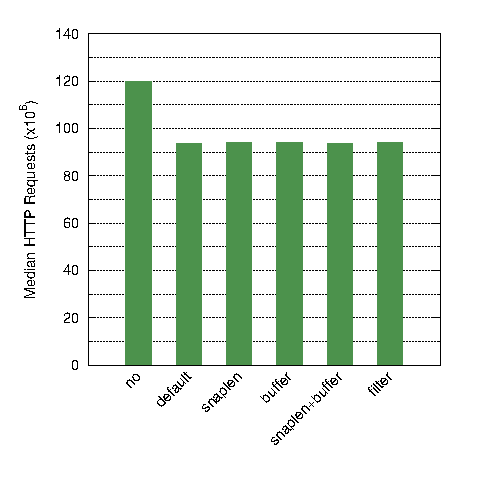
\includegraphics[width=0.5\textwidth]{images/requests}
    \caption{Anzahl der von wrk gesendeten HTTP Requests}\label{fig:results}
\end{figure}

Wie in Abbildung~\ref{fig:results} zu erkennen ist nimmt die Anzahl der
gesendeten HTTP Requests von wrk stark ab sobald tcpdump parallel zum Webserver
betrieben wird. Dabei kommt es zu eine Reduzierung der Requests um circa 25~\%
von rund 120 Million auf rund 90 Million Requests. Dies kann durch die erhöhte
Last auf dem ib6 Server erklärt werden. Zum einen werden nun alle Requests von
zwei Sockets verarbeiten. Außerdem teilen sich der Webserver und tcpdump nun
die verfügbaren Rechenkapazität auf dem Server. Weiterhin ist zu erkennen,
dass dieser Einfluss nahe zu konstant für alle Messungen mit tcpdump ist.

\begin{figure}
  \begin{subfigure}[b]{0.5\textwidth}
    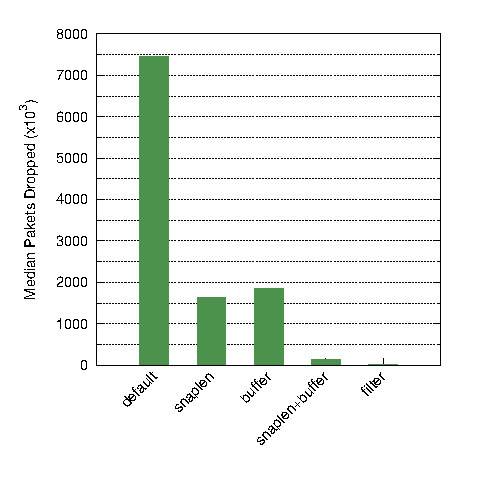
\includegraphics[width=\textwidth]{images/dropped}
    \caption{Anzahl der Pakete die vor tcpdump verloren wurden}\label{fig:dropped}
  \end{subfigure}
  %
  \begin{subfigure}[b]{0.5\textwidth}
    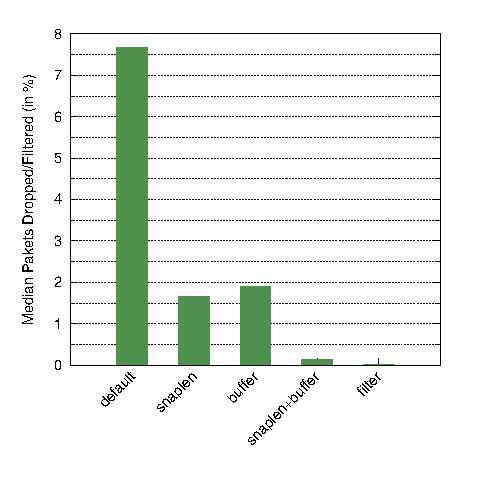
\includegraphics[width=\textwidth]{images/dropped-percentage}
    \caption{Prozentuale Anzahl der Pakete die vor tcpdump verloren wurden}\label{fig:dropped-percentage}
  \end{subfigure}
\caption{Paketverlust bevor tcpdump die Pakete auswerten konnte}\label{fig:results}
\end{figure}

In Abbildung~\ref{fig:dropped} ist die Anzahl der von tcpdump verloren Pakete
gezeigt. Zusätzlich zeigt~\ref{fig:dropped-percentage} den prozentualen Anteil
der verloren Paket von den empfangen Paketen.  Es zeigt sich das der
Paketverlust im Szenario \texttt{default} am Höchsten ist. Und das durch die
Anpassung der tcpdump Parameter eine starke Verbesserung erzielt werden kann.
Es scheint das die Reduzierung der aufgezeichneten Paketgröße einen größeren
Einfluss hat als eine Erhöhung des Empfangsbuffers. Dies kann dadurch erklärt
werden, dass die Paketgröße sehr stark reduziert wurde, von 65535 auf 142
Bytes. Zwar wurden keine Pakete versendet, welche 65535 Bytes groß sind,
allerdings entscheidet diese Größe wie libpcap den Ring Empfangsbuffer
aufteilt. Dabei geht es von der größt möglichsten Paketgröße aus. Mit einer
geringen Paketgrößte kann somit der vorhanden Buffer besser genutzt werden.
Die Kombination der beiden Parameter führte zu eine Reduzierung der verloren
Pakete von rund 98~\% im Vergleich zu dem \texttt{default} Szenario. So wurden
im Szenario \texttt{snaplen+buffer} nur noch 0.145~\% der empfangen Paket
verloren. Im Letzten Szenario \texttt{filter} konnte noch einmal eine
Verbesserung durch den optimierten Filter erzielt werden, hierbei sank die Zahl
der verloren Pakete auf 0.004~\%. Somit konnten fast alle Pakete bei einer Last
von rund 300.000 Requests pro Sekunde aufgezeichnet werden.

\clearpage
\section{Zusammenfassung}
\label{sec:zusammenfassung}

In dieser Arbeit wurde untersucht, wie tcpdump/libpcap Netzwerkpakete filtert
und aufzeichnet. Dazu wurde zu erst gezeigt, wie ein TCP Paket durch den Linux
Netzwerkstack verarbeitet wird. Dabei wurden die möglichen Ursachen für den
Paketverlust von tcpdump erklärt. Anschließend wurde ein Messkonzept erstellt,
um die Auswirkung dieser Punkte zu untersuchen. Die daraus resultierenden
Messungen bestätigten die Erwartung, dass diese Parameter entscheidend für die
Anzahl der verlorenen Pakete sind.

Es zeigte sich das es sehr wahrscheinlich zu Paketverlusten kommen kann, wenn
tcpdump zum Aufzeichnen von sehr hohem Netzwerkverkehr genutzt werden soll.
Allerdings kann diese Problem durch gezielte Auswahl der tcpdump Einstellungen
reduziert werden. Wie spezifisch die Einstellungen gewählt werden können hängt
vom jeweiligen Use Case ab. So konnte für den hier diskutierten Einsatzzweck,
der HTTP Lastverteilung, sehr spezifische Einstellungen vorgenommen werden.
Soll jedoch zum Beispiel der komplette TCP Verkehr von mehreren Anwendungen
aufgezeichnet werden, zum Beispiel für Intrusion Detection, dann muss ein recht
grober Filter gewählt werden und ein großer Teil des Paketes aufgezeichnet
werden.

Zusammenfassend konnte gezeigt werden, dass tcpdump zum Aufzeichnen von HTTP
Requests genutzt werden kann, sofern die Einstellungen auf diesen speziellen
Einsatzzweck optimiert werden. Außerdem sollte tcpdump nicht parallel auf dem
System betrieben wird, welches unter Last steht, da es einen Einfluss auf die
Leistung des Systems hat. Daher wäre es zu empfehlen das tcpdump Monitoring auf
einem dedizierten System durchzuführen. Dies ist auch deshalb zu empfehlen,
weil eine Weiterverarbeitung der tcpdump Aufzeichnung nötig ist, welche in
dieser Arbeit nicht betrachtet wurde.


\clearpage

%% BACKMATTER
\clearpage
\backmatter
% biblography
\nocite{*}
%\bibliographystyle{siam}
\bibliographystyle{gerplain}
\bibliography{bib/references}
\clearpage
% appendix
\appendix

\section{Konfigurationen}
\label{sec:konfigurationen}

\lstinputlisting[caption={Konfiguration von nginx auf ib6},label={lst:nginx}]{listings/nginx.conf}

\lstinputlisting[caption={Limits von ib5 und ib6 (ulimit)},label={lst:ulimit}]{listings/ulimit.conf}
\clearpage
\lstinputlisting[caption={Konfiguration der Netzwerkkarten von ib5 und ib6 (ethtool)},label={lst:ethtool}]{listings/ethtool.conf}

\clearpage
\section{Messskript}
\label{sec:messskript}

\lstinputlisting[caption={Skript zum Automatisieren der Messungen},label={lst:bench-auto},language=bash,numbers=left]{listings/bench-auto.sh}

\clearpage
\section{Messwerte}
\label{sec:messwerte}

\begin{table}[H]
  \centering
  \bgroup
  \def\arraystretch{1.2}
  \begin{tabular}{crrrrr}
      & \textbf{Requests} & \textbf{Requests/s} & \textbf{Filtered} & \textbf{Dropped} & \textbf{Dropped \%} \\\hline\hline
      1 & 119903581 & 399653,93 & - & - & - \\\hline
      2 & 120376044 & 401229,17 & - & - & - \\\hline
      3 & 120268758 & 400880,73 & - & - & - \\\hline
      4 & 119940796 & 399784,83 & - & - & - \\\hline
      5 & 120069354 & 400217,48 & - & - & - \\\hline
      6 & 119927287 & 399735,63 & - & - & - \\\hline
      7 & 120273002 & 400894,69 & - & - & - \\\hline
  \end{tabular}
  \egroup
  \caption{Messwerte für das Szenario \texttt{no}}\label{tab:messwerte-no}
\end{table}

\begin{table}[H]
  \centering
  \bgroup
  \def\arraystretch{1.2}
  \begin{tabular}{crrrrr}
      & \textbf{Requests} & \textbf{Requests/s} & \textbf{Filtered} & \textbf{Dropped} & \textbf{Dropped \%} \\\hline\hline
      1 & 93839932 & 312735,33 & 97637565 & 8000042 & 8,194~\%\\\hline
      2 & 94485540 & 314891,25 & 98306066 & 8334649 & 8,478~\%\\\hline
      3 & 93728797 & 312360,77 & 97520639 & 7030017 & 7,209~\%\\\hline
      4 & 93412256 & 311292,88 & 97190374 & 7446903 & 7,662~\%\\\hline
      5 & 92544907 & 308420,4 & 96289568 & 7288170 & 7,569~\%\\\hline
      6 & 94540226 & 315071,23 & 98364247 & 8474911 & 8,616~\%\\\hline
      7 & 93161788 & 310471,57 & 96933477 & 6717941 & 6,930~\%\\\hline
  \end{tabular}
  \egroup
  \caption{Messwerte für das Szenario \texttt{default}}\label{tab:messwerte-default}
\end{table}

\begin{table}[H]
  \centering
  \bgroup
  \def\arraystretch{1.2}
  \begin{tabular}{crrrrr}
      & \textbf{Requests} & \textbf{Requests/s} & \textbf{Filtered} & \textbf{Dropped} & \textbf{Dropped \%} \\\hline\hline
      1 & 93361461 & 311133,8 & 97139116 & 1638937 & 1,687~\%\\\hline
      2 & 94297388 & 314260,2 & 98111218 & 1142023 & 1,164~\%\\\hline
      3 & 93455367 & 311449,63 & 97234642 & 2256178 & 2,320~\%\\\hline
      4 & 94018148 & 313314,12 & 97820731 & 1224453 & 1,252~\%\\\hline
      5 & 94144165 & 313743,49 & 97952561 & 1806995 & 1,845~\%\\\hline
      6 & 94576465 & 315186,97 & 98400914 & 1634344 & 1,661~\%\\\hline
      7 & 94243027 & 314073,82 & 98053289 & 1608101 & 1,640~\%\\\hline
  \end{tabular}
  \egroup
  \caption{Messwerte für das Szenario \texttt{snaplen}}\label{tab:messwerte-snaplen}
\end{table}

\begin{table}[H]
  \centering
  \bgroup
  \def\arraystretch{1.2}
  \begin{tabular}{crrrrr}
      & \textbf{Requests} & \textbf{Requests/s} & \textbf{Filtered} & \textbf{Dropped} & \textbf{Dropped \%} \\\hline\hline
      1 & 94479121 & 314868,26 & 98301445 & 3138511 & 3,193~\%\\\hline
      2 & 93174474 & 310509,97 & 96945422 & 1464062 & 1,510~\%\\\hline
      3 & 94197335 & 313920,03 & 98005865 & 1860171 & 1,898~\%\\\hline
      4 & 94523845 & 315006,2 & 98346962 & 2196551 & 2,233~\%\\\hline
      5 & 94215312 & 313968,29 & 98025862 & 1768006 & 1,804~\%\\\hline
      6 & 93714952 & 312318,19 & 97506245 & 1445038 & 1,482~\%\\\hline
      7 & 93451164 & 311448,09 & 97232458 & 2033839 & 2,092~\%\\\hline
  \end{tabular}
  \egroup
  \caption{Messwerte für das Szenario \texttt{buffer}}\label{tab:messwerte-buffer}
\end{table}

\begin{table}[H]
  \centering
  \bgroup
  \def\arraystretch{1.2}
  \begin{tabular}{crrrrr}
      & \textbf{Requests} & \textbf{Requests/s} & \textbf{Filtered} & \textbf{Dropped} & \textbf{Dropped \%} \\\hline\hline
      1 & 93514281 & 311646,27 & 97298231 & 102277 & 0,105~\%\\\hline
      2 & 94436463 & 314707,05 & 98255678 & 142459 & 0,145~\%\\\hline
      3 & 93635020 & 312040,81 & 97422724 & 460590 & 0,473~\%\\\hline
      4 & 93659731 & 312103,79 & 97448350 & 14219 & 0,015~\%\\\hline
      5 & 94041647 & 313395,65 & 97844574 & 279299 & 0,285~\%\\\hline
      6 & 93608679 & 311969,3 & 97396242 & 330139 & 0,339~\%\\\hline
      7 & 92847251 & 309425,47 & 96604390 & 0 & 0,000~\%\\\hline
  \end{tabular}
  \egroup
  \caption{Messwerte für das Szenario \texttt{snaplen+buffer}}\label{tab:messwerte-snaplen-buffer}
\end{table}

\begin{table}[H]
  \centering
  \bgroup
  \def\arraystretch{1.2}
  \begin{tabular}{crrrrr}
      & \textbf{Requests} & \textbf{Requests/s} & \textbf{Filtered} & \textbf{Dropped} & \textbf{Dropped \%} \\\hline\hline
      1 & 93881869 & 312874,77 & 93883778 & 4893 & 0,005~\%\\\hline
      2 & 93082658 & 310188,31 & 93084571 & 3613 & 0,004~\%\\\hline
      3 & 94126289 & 313676,56 & 94128018 & 20014 & 0,021~\%\\\hline
      4 & 94240703 & 314049 & 94242269 & 2534 & 0,003~\%\\\hline
      5 & 92784745 & 309215,6 & 92786720 & 0 & 0,000~\%\\\hline
      6 & 94166541 & 313826,58 & 94168634 & 23905 & 0,025~\%\\\hline
      7 & 94220654 & 314003,73 & 94222585 & 2806 & 0,003~\%\\\hline
  \end{tabular}
  \egroup
  \caption{Messwerte für das Szenario \texttt{filter}}\label{tab:messwerte-filter}
\end{table}


%\listoftables
%\listoffigures
%\listofalgorithms



\end{document}
